\chapter{Wykład 15. Zarządzanie kontraktami w projekcie informatycznym}

\section{Formy wynajmu prac}
% strona 13

Z powodu niewielkich rozmiarów naszej firmy, a także braku specjalistów z niektórych dziedzin postanowiliśmy zlecić część zadań innym firmom. Dwa główne zadanie z którymi związane będzie zlecenie prac to opracowanie i stworzenie szaty graficznej dla naszego produktu, a także zapewnienie oraz utrzymanie serwerów na potrzeby naszego przedsiębiorstwa. Dla naszej firmy proponujemy następujące formy wynajmu prac:
\begin{itemize}
\item Najlepsze osiągalne rozwiązania (best-of-breed) – w każdym obszarze planujemy rozważyć zlecenie zadań związanych z nim na zewnątrz, albo pozostawienie ich wewnątrz firmy. Kupowanie rozwiązań dla różnych obszarów od różnych firm pozwoli nam zapewnić najlepsze dla przedsiębiorstwa rozwiązanie.
\item Partnerstwo – zawarcie umowy z inną firmą zajmującą się szeroko pojętą grafiką, pozwoli nam zapewnić szatę graficzną naszego produktu na wysokim poziomie, a także przetransferować ryzyko związane z brakiem grafików w naszym zespole.
\item Outsourcing – planujemy oddelegować do zewnętrznej firmy zadań związanych z dostarczeniem i utrzymaniem serwera na potrzeby naszego przedsiębiorstwa.
\end{itemize}

% ===========================================================================

\section{Szkic kontraktu}
% strona 31

Szkic kontraktu znajduje się na następnych stronach.

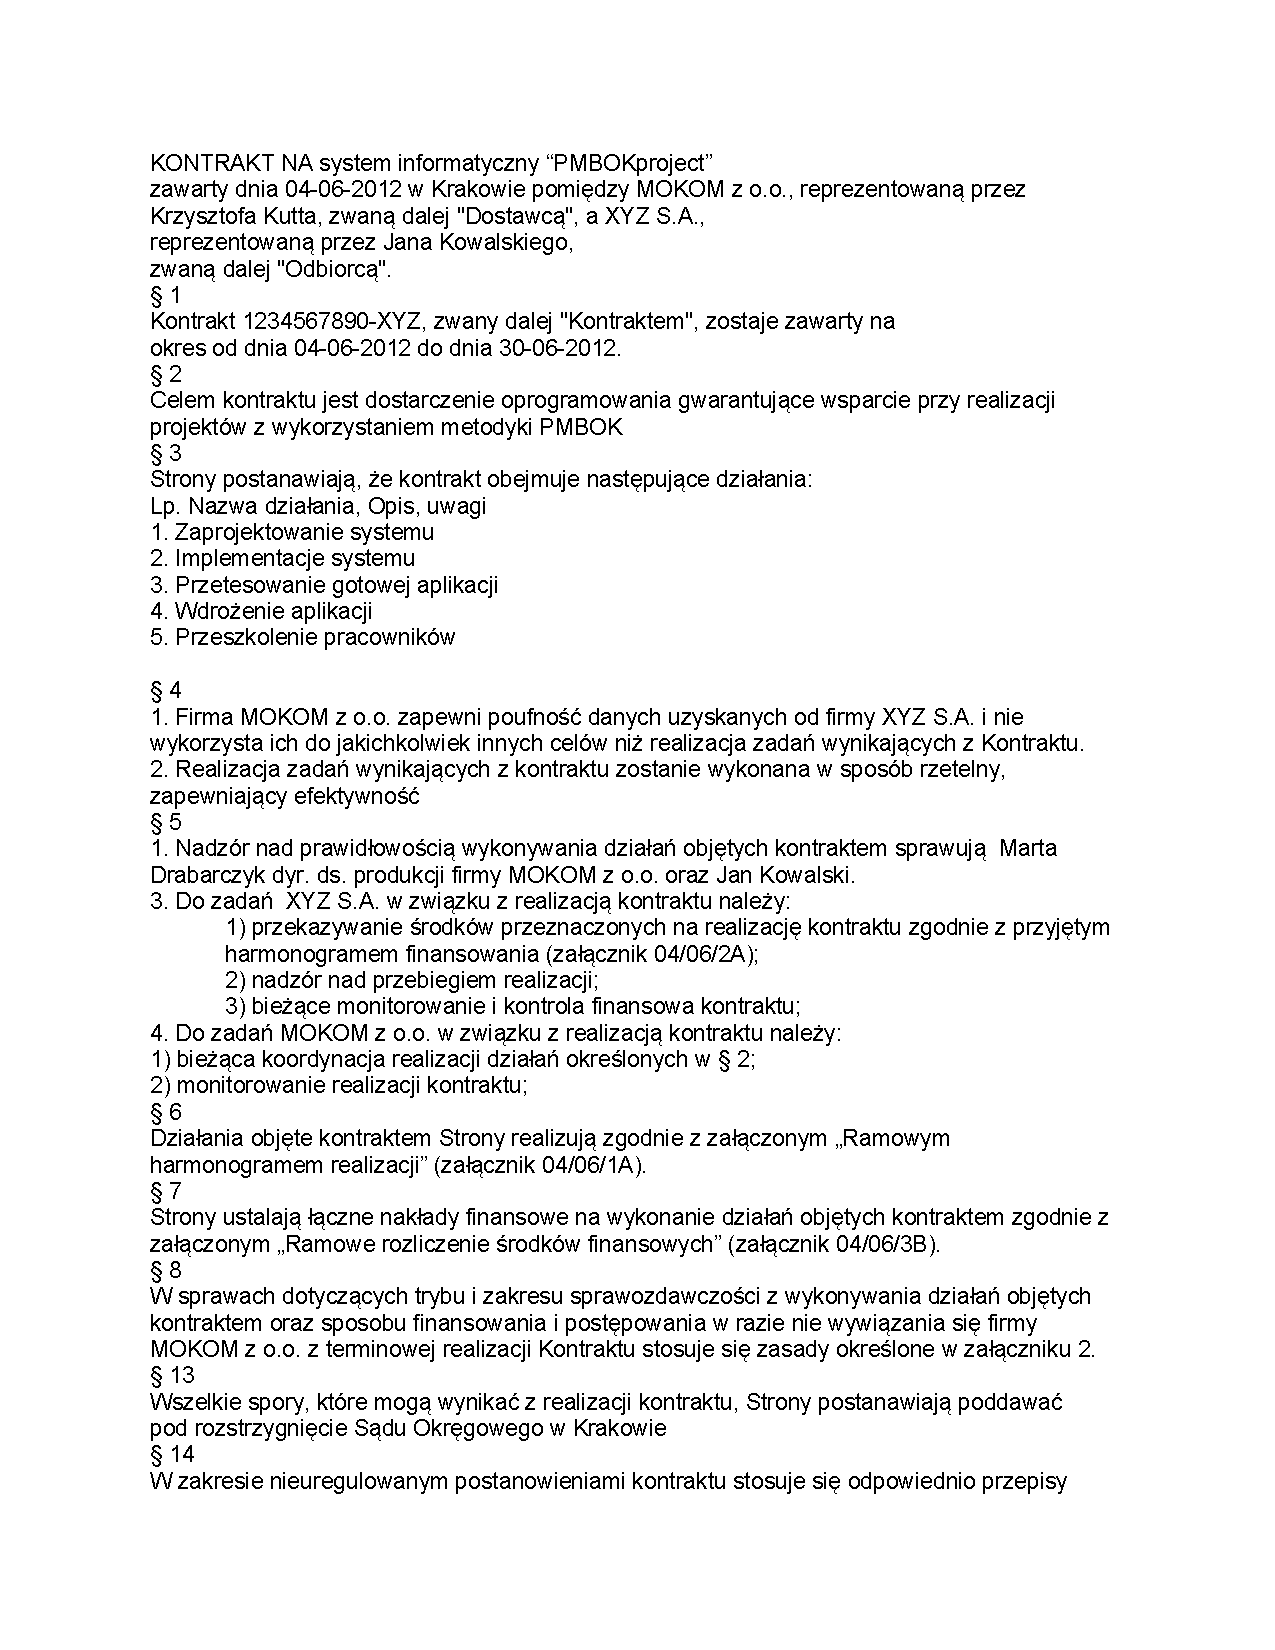
\includepdf[pages=-]{szkicKontraktu.pdf}

\clearpage

% ===========================================================================

\section{Wybór prac, które należy zlecić. Wybór dostawcy}
% strona 50

\subsection*{Można zlecić prace, gdy:}
\begin{enumerate}
\item Kontrola nie jest dla nas największym priorytetem
\item Praca nie wiąże się z dostępem do poufnych informacji i procedur
\item Brakuje nam pracowników, bądź innych zasobów (np komputerów)
\item Mamy odpowiednie środki finansowe
\item Zakupienie / zlecenie będzie tańsze niż samodzielna produkcja
\item Funkcjonalności nie są kluczowe dla projektu
\item Mamy niewystarczające doświadczenie
\end{enumerate}

\subsection*{Kryteria wyboru dostawcy}
\begin{enumerate}
\item Jakość
\item Czas
\item Koszt (produkcji i utrzymania), w porównaniu do naszych możliwości finansowych
\item Niezawodność (np. poprzednie zlecenia wykonane przez tego dostawcę)
\item Dokładne zrozumienie potrzeb przez dostawcę
\item Ryzyko
\item Gwarancja
\item Referencje
\item Lokalizacja (w okolicy naszej firmy, czy na drugim końcu świata?)
\end{enumerate}

\clearpage

% ===========================================================================

\section{Wybór kontraktu dla organizacji oraz podwykonawców}
% strona 70

Zdecydowaliśmy się na następujące kontrakty dla naszego przedsiębiorstwa oraz dla wybranych przez nas podwykonawców:
\begin{itemize}
\item Umowa z ustaloną ceną zwiększoną opłatę motywacyjną - FPIF (Fixed Price Incentive Fee); ten typ umowy zawarty zostanie pomiędzy naszym przedsiębiorstwem, a firmą zamawiającą projekt. Zdecydowaliśmy się na ten typ kontraktu ponieważ jesteśmy w stanie już na początku oszacować koszty projektu, a także taka forma umowy pomaga motywować pracowników do kontrolowania rzeczywistych kosztów. Wadami tego typu kontraktu są na pewno ryzyko niechęci zaakceptowania produktu jako skończonego przez klienta oraz stosunkowo duże ryzyko. Dodatkową zaletą jest także możliwość zwiększonej opłaty motywacyjnej.
\item Umowa z wiążącą stałą ceną - FFP (Firm Fixed Price); ten typ kontraktu zostanie zawarty pomiędzy naszą firmą, a przedsiębiorstwem odpowiedzialnym za zapewnienie nam serwerów. Zaletami w tym przypadku są małe koszty zarządzania kontraktem oraz znajomość całego kosztu już na początku zawarcia kontraktu, wadami natomiast niepewność otrzymania dokładnie tego co potrzebujemy.
\item Umowy z refundowanymi kosztami powiększonymi o stałą opłatę (CPFF – Costs-plus-fixed-fee);  ta umowa zostanie zawarta z firmą dostarczającą szatę graficzną do naszego produktu. Zdecydowaliśmy się na ten typ kontraktu ponieważ gwarantuje on niższe koszty niż umowa z stałą ceną, a także uproszcza deklarację zakresu prac. Wadami są natomiast nieuwzględnienie ewentualnych kosztów ryzyka, a także mała motywacja u firmy dostarczającej nam usługi do kontrolowania swoich kosztów.
\end{itemize}

